\section{Vorgehensmodell}
\subsection{Rational Unified Process (RUP)}

\begin{figure}[H]
\centering
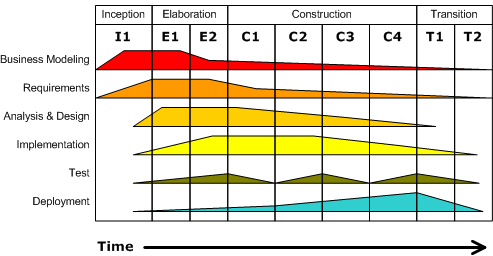
\includegraphics[width=300pt]{images/rup.png}
\caption[RUP]{RUP}
\end{figure}

Das Projekt OSM Crosswalk Detection führten wir mit dem Vorgehensmodell RUP \cite{RUP} aus.
Dies ist eine iterative Art um Softwareprojekt anzugehen. RUP kennt die Phasen:

\begin{itemize}
	\item Inception, Elaboration, Construction, Transition
\end{itemize}

Um eine feinere Aufteilung zu haben, unterteilten wir die Elaboration, sowie die Construction in je zwei Hälften. 

\subsubsection{Fazit}
Wir hatten Mühe unserem Projekt ein RUP Stempel auf zu drücken, da wir bei der Evaluation der Algorithmen immer wieder grosse Teile unserer Lösung überdenken und auf den Kopf stellen mussten. Es wurde viel geschriebener Code wieder über den Haufen geworfen. Weiter war es schwierig den Phasen gerecht zu werden, nur mit vielen Überstunden konnte am Ende der Elaboration ein Prototyp präsentiert werden, der ein angemessenes Resultat lieferte. Im Nachhinein hätte sich ein agilieres Vorgehensmodell wie Scrum oder ähnlich vielleicht besser bewährt.
 

